\documentclass[aspectratio=169]{beamer}
\usepackage{pgf}
\usepackage{multimedia}
\usepackage{colortbl,tabularx,mathrsfs,calligra,xcolor}
\usepackage{amsmath,amsfonts,amssymb,amsthm}
\usepackage{ragged2e}
\usepackage{setspace}
\usepackage{filecontents}
\usepackage{caption}
\usepackage{subcaption}
\usepackage{contour}
\usepackage{animate}
\usepackage{fancybox}
\usepackage{wrapfig}
\usepackage{multirow}
\usepackage{multicol}
\usepackage{pgfplots, tkz-euclide,calc}
    \usetikzlibrary{patterns,snakes,shapes.arrows,shapes.geometric,arrows}
\usepackage{listings}
\usepackage{enumitem}
\usepackage{pifont}
\usepackage[scaled]{berasans}
    \renewcommand*\familydefault{\sfdefault}  %% Only if the base font of the document is to be sans serif
\usepackage[T1]{fontenc}
\usepackage{hyperref}
\hypersetup{
    filecolor=magenta,      
    urlcolor=cyan,
    pdftitle={Overleaf Example},
    pdfpagemode=FullScreen,
    }
\renewcommand*\familydefault{\sfdefault} %% Only if the base font of the document is to be sans serif

\graphicspath{{C:/Users/teoso/OneDrive/Documents/Asisten Dosen & Lab/Asisten Laboratorium/Alpro 1/PPT/Graphicx/}}

\definecolor{HIMAmuda}{HTML}{01D1FD}
\definecolor{HIMAtua}{HTML}{02016A}
\definecolor{HIMAabu}{HTML}{CBCBCC}
\definecolor{PastelGreen}{HTML}{77DD77}
\definecolor{pgray}{rgb}{0.5,0.5,0.5}
\definecolor{pblue}{rgb}{0.13,0.13,1}
\definecolor{pgreen}{rgb}{0,0.5,0}
\definecolor{pred}{rgb}{0.9,0,0}
\definecolor{pgrey}{rgb}{0.46,0.45,0.48}
\definecolor{pcyan}{HTML}{D4EFFC}
\definecolor{lblue}{HTML}{00AEEF}
\definecolor{input}{HTML}{AAE1FA}
\definecolor{bg}{rgb}{0.95, 0.95, 0.92}
\definecolor{vscode}{HTML}{282A36}

\usetheme{Madrid}

\setbeamercolor{palette primary}{bg=HIMAtua,fg=white}
\setbeamercolor{palette secondary}{bg=HIMAmuda,fg=black}
\setbeamercolor{palette tertiary}{bg=HIMAabu,fg=black}
\setbeamercolor{palette quaternary}{bg=HIMAmuda,fg=white}
\setbeamercolor{structure}{fg=HIMAmuda} % itemize, enumerate, etc
\setbeamercolor{section in toc}{fg=HIMAtua} % TOC sections
\setbeamercolor{block title alerted}{fg=white,bg=magenta}
\setbeamercolor{block body alerted}{fg=black!90,bg=pink}

\usefonttheme{professionalfonts}
\setbeamertemplate{theorems}[numbered]
\setbeamertemplate{itemize items}[circle]

\usebackgroundtemplate{%
\tikz[overlay,remember picture] \node[opacity=0.1, at=(current page.center)]{\includegraphics[width=\paperwidth]{plana class}};
}

\renewcommand\thesubfigure{\arabic{subfigure}}
\newtheorem*{funfact}{Fun Fact}
\newtheorem*{definisi}{Definisi}
\newtheorem{teorema}{Teorema}
\theoremstyle{definition}
\newtheorem{latihan}{Latihan}
\newtheorem*{contoh}{Contoh}
\newtheorem*{masalah}{Masalah}
\newcommand{\R}{\mathbb{R}}

\AtBeginEnvironment{contoh}{%
    \setbeamercolor{block title}{use=example text,fg=white,bg=example text.fg!75!black}
    \setbeamercolor{block body}{parent=normal text,use=block title example,bg=block title example.bg!10!bg}
}

\AtBeginEnvironment{funfact}{%
  \setbeamercolor{block title}{fg=white,bg=PastelGreen!50!HIMAmuda} % Set title background to pastel green and text to white
  \setbeamercolor{block body}{parent=normal text,bg=PastelGreen!50!HIMAmuda!30!white} % Set body background to a lighter pastel green
}
\AtBeginEnvironment{definisi}{
    \setbeamercolor{block title}{fg=white,bg=HIMAtua}
    \setbeamercolor{block body}{parent=normal text,bg=HIMAtua!30!white}
}
\AtBeginEnvironment{teorema}{
    \setbeamercolor{block title}{bg=darkgray,fg=white}
    \setbeamercolor{block body}{parent=pallette tertiary,bg=HIMAabu!30!white}
}
\AtBeginEnvironment{latihan}{%
  \setbeamercolor{block title}{fg=white,bg=PastelGreen} % Set title background to pastel green and text to white
  \setbeamercolor{block body}{parent=normal text,bg=PastelGreen!30!white} % Set body background to a lighter pastel green
}
\AtBeginEnvironment{masalah}{%
  \setbeamercolor{block title}{fg=white,bg=teal} % Set title background to pastel green and text to white
  \setbeamercolor{block body}{parent=normal text,bg=teal!30!white} % Set body background to a lighter pastel green
}

\renewcommand{\arraystretch}{1.3}
\renewcommand{\lstlistingname}{Kode}

\usepackage{listings}

\lstdefinestyle{standard}{
    language            = Java,
    showspaces          = false,
    showtabs            = false,
    breaklines          = true,
    showstringspaces    = false,
    breakatwhitespace   = true,
    commentstyle        = \color{pgray},
    keywordstyle        = \color{pblue},
    stringstyle         = \color{pgreen},
    basicstyle          = \footnotesize\ttfamily,
    frame               = shadowbox,
    backgroundcolor     = \color{brown!10!white},
    escapeinside        = {(*}{*)},
    numbers             = left, % {none, left, right}
    numberstyle         = \scriptsize\color{lightgray},
    numbersep           = -8pt,
    rulesepcolor        =\color{brown!50!black}
    }

\lstdefinestyle{output}{
    language=Java,
    backgroundcolor     =\color{vscode},
    basicstyle          =\footnotesize\ttfamily\color{white},
    frame               =shadowbox,
    escapeinside        ={(*}{*)},
    showspaces          =false,
    showtabs            =false,
    breaklines          =true,
    showstringspaces    =false,
    breakatwhitespace   =true,
    rulesepcolor        =\color{HIMAtua!50!white},
    rulecolor           =\color{HIMAtua!50!white},
    numbers             =none,
    }

\lstset{style=standard}

\tikzstyle{startstop} = [rectangle, rounded corners, 
minimum width=2cm, 
minimum height=1cm,
text centered, 
draw=black, 
fill=pink]

\tikzstyle{io} = [trapezium, 
trapezium stretches=true, % A later addition
trapezium left angle=70, 
trapezium right angle=110, 
minimum width=2cm, 
minimum height=1cm, text centered, 
draw=black, fill=HIMAmuda]

\tikzstyle{process} = [rectangle, 
minimum width=2cm, 
minimum height=1cm, 
text centered, 
text width=2cm, 
draw=black, 
fill=HIMAabu]

\tikzstyle{decision} = [diamond, 
minimum width=2cm, 
minimum height=1cm, 
text centered, 
draw=black, 
fill=PastelGreen]
\tikzstyle{arrow} = [thick,->,>=stealth]

\newcommand{\enter}{\raisebox{-1.8pt}{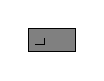
\begin{tikzpicture}[scale=0.3]
    \draw[thin,fill=gray] (0,0) rectangle (2,1);
    \draw (0.3,0.3) -- (0.7,0.3)--(0.7,0.6);     
\end{tikzpicture}}}

\newcommand{\inputscan}[1]{\raisebox{0pt}[1pt]{\colorbox{darkgray}{#1}}}

\newcommand{\inlineitem}{%
\leavevmode\usebeamertemplate{itemize item}
}

\author[Tew \& Haf]{Hafidz Mulia\\Teosofi Hidayah Agung}
\date{28 Oktober 2024}
\title[Alpro 1 - Week 7]{Fungsi/Method}
\institute[Matematika ITS]{Departemen Matematika\\ Institut Teknologi Sepuluh Nopember}
\titlegraphic{{\includegraphics[scale=0.02]{M.png}$\quad$\includegraphics[scale=0.2]{Provicom.png}}}

\begin{document}
    {\usebackgroundtemplate{
        \tikz[overlay,remember picture] \node[opacity=0.2, at=(current page.center)]{\includegraphics[width=\paperwidth]{bg_2}};}
    \begin{frame}
        \titlepage
    \end{frame}
    }

    \AtBeginSection{
    {\usebackgroundtemplate{
     \tikz[overlay,remember picture] \node[opacity=0.1, at=(current page.center)]{\includegraphics[width=\paperwidth]{Java code}};}
    \begin{frame}{Daftar isi}
        \tableofcontents[currentsection]
        \begin{tikzpicture}[overlay, remember picture] 
            \node at ([yshift=.5cm]current page.south east) [
                anchor = south east, 
                ] {
            \animategraphics[autoplay,loop,width=0.2\textwidth]{30}{Arisu Dance/Arisu Dance-}{0}{186}
            };
        \end{tikzpicture}
    \end{frame}}
    }

    \begin{frame}
        \begin{masalah}
            \textit{Copy-paste} memanglah hal yang sangat mudah dilakukan namun juga melelahkan jika yang akan di-\textit{copas} terlalu banyak. Misalkan kita memiliki program yang memiliki 100 baris kode dan kita ingin mengulangnya sebanyak 10 kali. Tentu saja kita tidak akan menulis ulang program tersebut sebanyak 10 kali. Oleh karena itu, kita memerlukan suatu cara agar program tersebut dapat dijalankan berkali-kali tanpa harus menulis ulang program tersebut.
        \end{masalah}
    \end{frame}

    \section{Fungsi}
    \begin{frame}
        \frametitle{\insertsection}
        \begin{definisi}
            \textbf{Fungsi} secara umum didefinisikan sebagai hubungan/pemetaan antara himpunan input dan himpunan output.
        \end{definisi}
        \begin{contoh}
            Misalkan $A=\{\text{Fuad, Disty, Yusuf}\}$  dan $B=\{\text{D, F, Y}\}$. Kemudian Didefinisikan fungsi $f:A\to B$ dengan aturan sebagai berikut:\\~\\
            \begin{columns}
                \begin{column}{0.5\textwidth}
                    $\blacktriangleright$ $f:=\text{Huruf pertama dari nama di } A$
                    \begin{itemize}[label=$\bullet$]
                        \item Fuad $\mapsto$ F
                        \item Disty $\mapsto$ D
                        \item Yusuf $\mapsto$ Y
                    \end{itemize}
                \end{column}
                \begin{column}{0.5\textwidth}
                    $\blacktriangleright$ $f:=\text{Huruf terakhir dari nama di } A$
                    \begin{itemize}[label=$\bullet$]
                        \item Fuad $\mapsto$ D
                        \item Disty $\mapsto$ Y
                        \item Yusuf $\mapsto$ F
                    \end{itemize}
                \end{column}
            \end{columns}
        \end{contoh}
    \end{frame}

    \begin{frame}
        \frametitle{\insertsection}
        \begin{alertblock}{Perhatikan}
            Input yang diberikan kepada fungsi haruslah sesuai dengan definisi fungsi parameter tersebut. Jika tidak, maka akan terjadi error. Misalkan saja kita berikan input berupa angka pecahan kepada fungsi diatas maka jelas sekali si fungsi akan bingung.
        \end{alertblock}
    \end{frame}

    \section{Method}
    \begin{frame}
        \frametitle{\insertsection}
        \begin{definisi}
            \textbf{Method} adalah blok kode yang dirancang untuk melakukan tugas tertentu dan dapat dipanggil kapan saja dalam program. Penggunaan method membuat kode lebih terstruktur, dapat digunakan kembali (\textit{reusable}), dan lebih mudah dibaca.
        \end{definisi}
        \begin{block}{Method Java}
            Berdasakan asal atau sumbernya bisa dibagi menjadi dua jenis:
            \begin{itemize}[label=$\blacktriangleright$]
                \item \textbf{Built-in Method} adalah method yang sudah disediakan oleh Java. Contoh: \texttt{System.out.println()}, \texttt{Math.abs()}, \texttt{Math.sqrt()}, dll.
                \item \textbf{User-defined Method} adalah method yang dibuat oleh pengguna. Inilah yang akan kita pelajari.
            \end{itemize}
        \end{block}
    \end{frame}

    \subsection{Struktur Method}
    \begin{frame}[fragile]
        \frametitle{\insertsection}
        \framesubtitle{\insertsubsection}
        \begin{lstlisting}[caption={Struktur Method}]
    <access_modifier> <return_type> <method_name>(list_of_parameters) {
        // Body of the method
        // Statements to be executed
        return <value>;
    }
        \end{lstlisting}
        \begin{block}{}
            \begin{itemize}[label=$\blacktriangleright$]
                \item \texttt{access\_modifier} adalah kata kunci yang menentukan tingkat akses method. Contoh: \texttt{public}, \texttt{private}, \texttt{protected}, dll.
                \item \texttt{return\_type} adalah tipe data yang akan dikembalikan oleh method. Jika method tidak mengembalikan nilai, gunakan tipe data \texttt{void}.
                \item \texttt{method\_name} adalah nama method yang akan digunakan.
                \item \texttt{parameters} adalah variabel yang diperlukan oleh method.
            \end{itemize}
        \end{block}
    \end{frame}

    \begin{frame}[fragile]
        \frametitle{\insertsection}
        \framesubtitle{\insertsubsection}
        \begin{alertblock}{Catatan}
            Yang wajib dibuat dalam method adalah \texttt{return\_type} dan \texttt{method\_name}. Sedangkan \texttt{parameters} dan \texttt{access\_modifier} adalah opsional.
        \end{alertblock}
        Contoh:
        \begin{lstlisting}
    public static void hello() {
        System.out.println("Hello, World!");
    }
        \end{lstlisting}
    bisa diubah menjadi
        \begin{lstlisting}
    static void hello() {
        System.out.println("Hello, World!");
    }
        \end{lstlisting}
    \end{frame}

    \subsection{Parameter}
    \begin{frame}[fragile]
        \frametitle{\insertsection}
        \framesubtitle{\insertsubsection}
        \begin{definisi}
            \textbf{Parameter} adalah variabel yang didefinisikan di dalam tanda kurung saat kita membuat sebuah method. Parameter digunakan untuk menerima data atau input dari luar method, sehingga method tersebut bisa bekerja berdasarkan nilai yang diberikan. Dengan kata lain, parameter memungkinkan kita untuk mengirimkan data yang berbeda setiap kali memanggil method yang sama, sehingga method tersebut bisa melakukan tugas yang lebih fleksibel.
        \end{definisi}
    \end{frame}

    \begin{frame}[fragile]
        \frametitle{\insertsection}
        \framesubtitle{\insertsubsection}
        \begin{lstlisting}[caption={Parameter pada Method}]
    returnType methodName(parameterType parameterName) {
        // kode di dalam method
    }
        \end{lstlisting}
        \begin{block}{Penjelasan}
            \begin{itemize}[label=$\blacktriangleright$]
                \item \texttt{parameterType} adalah tipe data dari parameter yang diterima method, seperti \texttt{int}, \texttt{double}, \texttt{String}, dll.
                \item \texttt{parameterName} adalah Nama variabel untuk parameter, yang akan digunakan sebagai referensi dalam method.
            \end{itemize}
            Paramater bisa lebih dari satu, dipisahkan dengan tanda koma.
        \end{block}
    \end{frame}

    \begin{frame}[fragile]
        \frametitle{\insertsection}
        \framesubtitle{\insertsubsection}
        \begin{lstlisting}[caption={Contoh Method berparameter}]
    public static void greet(String name) {
        System.out.println("Hello, " + name);
    }
        \end{lstlisting}
        \begin{lstlisting}
    public static void int f(double a, char b) {
        // Blok kode
        return int_type;
    }
        \end{lstlisting}
    \end{frame}

    \subsection{Pemanggilan Method}
    \begin{frame}
        \frametitle{\insertsection}
        \framesubtitle{\insertsubsection}
        \begin{block}{Memanggil Method}
            Method yang telah dibuat tidak akan berjalan jika tidak dipanggil. Untuk memanggil method, kita cukup menuliskan nama method tersebut di dalam method \texttt{main()} dan jangan lupa untuk memberikan tanda kurung "()" di belakang nama method.
        \end{block}
        \begin{exampleblock}{Perbedaan}
            Membedakan antara method dan variabel cukup mudah yaitu method selalu diakhiri dengan tanda kurung "()". Sedangkan variabel tidak.
        \end{exampleblock}
    \end{frame}


    \begin{frame}[fragile]
        \frametitle{\insertsection}
        \framesubtitle{\insertsubsection}
        \begin{lstlisting}[caption={Pemanggilan Method}]
    public class Method {
        public static void main(String[] args) {
            hello();
            hello();
            hello();
        }
        static void hello() {
            System.out.println("Hello, World!");
        }
    }
        \end{lstlisting}
        \begin{lstlisting}[style=output]
    Hello, World!
    Hello, World!
    Hello, World!
        \end{lstlisting}
    \end{frame}

    \begin{frame}[fragile]
        \frametitle{\insertsection}
        \framesubtitle{\insertsubsection}
        Disinilah kita bisa menggunakan \textit{syntax} \texttt{return} secara maksimal. 
        \begin{lstlisting}[caption={Penjumlahan Dua Bilangan}]
    public class Method {
        public static void main(String[] args) {
            int x = 10, y = 20, z = add(x, y);
            System.out.println("Hasil" +x +" + " +y +" = " +z);
        }
        public static int add(int a, int b) {
            return a + b;
        }
    }
        \end{lstlisting}
    \end{frame}

    \begin{frame}
        \frametitle{\insertsection}
        \framesubtitle{\insertsubsection}
        \begin{block}{Pertanyaan}
            \begin{itemize}[label=$\bullet$]
                \item Apa yang terjadi jika kita menghilangkan \texttt{return} pada method \texttt{add()}?
                \item Bisakah method \texttt{add()} langsung dipanggil di dalam \texttt{println}?
                \item Jika kita hanya menuliskan \texttt{add(x, y)} tanpa menyimpannya ke dalam variabel, apakah akan terjadi error?
            \end{itemize}
        \end{block}
    \end{frame}



    \section{Rekursif}
    \begin{frame}[fragile]
        \frametitle{\insertsection}
        \begin{definisi}
            \textbf{Rekrusif} adalah teknik pemrograman dimana suatu fungsi memanggil dirinya sendiri. ekursi adalah cara menyelesaikan masalah dengan memecah masalah besar menjadi sub-masalah yang lebih kecil dan lebih sederhana hingga mencapai kondisi dasar (atau \textit{base case}) yang dapat diselesaikan secara langsung tanpa rekursi lebih lanjut.
        \end{definisi}
        \begin{lstlisting}[caption={Salah satu struktur Rekrusif}]
    return_type method_name(parameters) {
        // Statements
        return method_name(another_parameters);
    }
        \end{lstlisting}
    \end{frame}

    \begin{frame}[fragile]
        \frametitle{\insertsection}
        \begin{alertblock}{Infinite Recursive}
            Rekursif pada dasarnya adalah pengulangan yang dilakukan oleh method itu sendiri. Oleh karena itu, dalam menggunakannya perlu diperhatikan agar tidak terjadi \textit{infinite recursive}.
        \end{alertblock}
        \begin{lstlisting}[caption={Infinite Recursive}]
    public static void infinite() {
        System.out.println("Infinite Recursive");
        infinite();
    }
        \end{lstlisting}
    \end{frame}

    \begin{frame}[fragile]
        \frametitle{\insertsection}
        \begin{contoh}
            Program untuk menghitung faktorial dari suatu bilangan.
        \end{contoh}
        \begin{lstlisting}[caption={Faktorial}]
    public class Method {
        public static void main(String[] args) {
            int n = 5;
            System.out.println("Faktorial dari " +n +" adalah " + factorial(n));
        }
        public static int factorial(int n) {
            if (n == 0 || n == 1) return 1;
            return n * factorial(n - 1);
        }
    }
        \end{lstlisting}
    \end{frame}

    \section{Latihan}
    \begin{frame}
        \begin{latihan}
            Buatlah program untuk menentukan mana diantara 2 bilangan yang terbesar ($\max(a, b)$) menggunakan method.
        \end{latihan}
        \begin{latihan}
            Buatlah program yang menerima input $n$ bilangan asli dan memunculkan output berupa segitiga pascal.
        \end{latihan}
        \begin{latihan}
            Buatlah program untuk menghitung jumlahan faktor dari bilangan bulat positif $n$.\\
            Contoh: $n=6$, maka faktornya adalah $1, 2, 3, 6$. Jumlahnya adalah $12$.
        \end{latihan}
    \end{frame}
\end{document}